% Chapter 6

\chapter{Conclusion} % Write in your own chapter title
\label{Chapter:Conclusion}
\lhead{Chapter 6. \emph{Conclusion}} % Write in your own chapter title to set the page header
\begin{center}
    \textit{``We gaze continually at the world and it grows dull in our perceptions. Yet seen from another's vantage point, as if new, it may still take the breath away.''}
    Alan Moore - Watchmen
\end{center}


This thesis describes $\steel$, the STastical sEmi-Empirical modeL, a model designed to use the empirical technique in a new fashion. The design of \steel allows for extremely fast, flexible and transparent testing of a variety of galaxy formation theories. The novelty introduced by the statistical dark matter accretion histories allow \steel to make predictions that would be limited with other traditional (discrete/non-statistical) numerical or analytic tools of galaxy formation. The foremost problem concerning galactic modelling on a cosmological scale is one of constraint is represented by the large number of physical processes at play at different scales and the limited knowledge in how to describe them. Complexity and uncertainty are built into models from all contributing aspects, from the dark matter simulations \cite[e.g.]{vandenBosch2018DisruptionFiction}, to observations \cite[e.g.]{Bernardi2017ComparingLight, Lapi2017StellarEquation, Leja2019AnSurvey}. Techniques have been developed to try to reduce the impact of these complexities, for example:
\begin{itemize}
    \item To reduce the need to build stellar mass from first principles following gas collapse. Abundance matching is used to create a mapping between galaxy stellar mass at the centre of a halo and the mass of the host halo itself at any redshift accessible by observations. In doing so it provides a robust framework to model the evolutionary tracks of galaxies following the growth of their host dark matter haloes.
    \item To remove tensions between conflicting observations such as the cosmic stellar mass density and cosmic star formation rate. Continuity modelling is used to predict the star formation rate using the evolution of the stellar mass function from high to low redshift. 
\end{itemize}

The impact of publication bias, the preferential publishing of positive and novel results is a known problem in academic disciplines \cite[e.g.]{Song2010DisseminationBiases}. It is unsurprising then that the number of papers that report new techniques or fits to data far outweigh those models which deconstruct the techniques to understand how our models work and document their limitations \cite[e.g.][]{vandenBosch2017DissectingSimulation, vandenBosch2018DisruptionFiction, Asquith2018CosmicModels}. Additionally, it can be expected that, for example, tuning of high parameter systems to create high fidelity matches to data, will generate a higher publication impact then equally important tools analysis. The design of \steel has been influenced by this culture. We prioritise the understanding of systematics and internal self consistency above that of fitting new features. Where new features are introduced they use modular and flexible modelling techniques that can be analysed independently.


\steel is statistical model and not a physical model, in this way is the antithesis of high resolution single galaxy or cluster simulations such as FIRE \cite{Hopkins2018FIRE-2Formation}. Galaxy modelling is often described as a spectrum from hydrodynamical, though semi-analytic and semi-empirical to mock catalogues produced via HOD. In this regime \steel can be thought of as occupying a space between traditional semi-empirical and HOD modelling. We retain the ability to track galaxy populations in redshift but forgo the tracking of discrete objects from step to step. Despite the antithetical nature of \steel to the hydrodynamical and non-statistical models it is not adversarial, used in conjunction with other techniques it will prove to be a valuable tool for the galaxy modelling community. 

\section{Pros and Cons of \steel as a Galaxy Model}
%successes of STEEL where other models fall down
%what if theoretically impossible in steel that other models can do

\steel has had the following major successes:
\begin{itemize}
    \item Reproduction of the statistical distribution of satellite galaxies in dark matter halos over a broad range of redshifts and halo masses, a challenge for traditional \LCDM models. (Chapter \ref{Chapter:GalDist})
    \item Identification of the inconsistencies between certain stellar mass functions and dark matter accretion histories produced by \LCDM cosmologies. (Chapter \ref{Chapter:GalGrowth})
    \item Derivation of the star formation rate from a new halo centric approach, consistent with cutting-edge observations.(Chapter \ref{Chapter:GalGrowth})
    \item Analysis of the systematic effect the estimation of stellar masses has on the observed galaxy pair fraction. (Chapter \ref{Chapter:GalPairs})
\end{itemize}
Each of the points listed above directly stems from the statistical approach of \steel to dark matter accretion histories. However, this technique loses individual galaxies that could be tracked through hydrodynamical, semi-analytic, and traditional semi-empirical models.

\steel is an exceptional tool for systematic modelling, by applying predictions to statistically significant volumes we are able to draw transparent conclusions about the way assumptions and models propagate into observed populations. Furthermore, Chapter \ref{Chapter:GalPairs} shows the potential of this systematic technique to track how changes to input propagate to output in a complex system, as shown with the pair fractions. Additionally, STEEL allows for fast,  effective, and precise testing of a variety of recipes for galaxy evolution, such as the formation of bulges via mergers and disc instabilities.

\section{Impact of \steel}
%how impactful is the work done with STEEL on the wider field?

\subsection{Modelling}

Creating another cosmological model acting on a discrete dark matter background has little value to add to the large number of competitive models already existing in empirical, \cite[e.g.][]{Rodriguez-Puebla2017ConstrainingProperties, Moster2018Emerge10, Behroozi2019UniverseMachine:010, Zavala2012}, analytic \cite[e.g.][]{Somerville2015StarGas, Guo2011FromCosmology, Fontanot2007ReproducingCosmogony, Zoldan2019TheEvolution} and, hydrodynamical \cite{Springel2018FirstClustering, Hopkins2018FIRE-2Formation, McAlpine2015TheCatalogues} regimes. The systematic statistical approach of \steel can be used to complement these models in two ways:
\begin{itemize}
    \item Pre-Processing: 
    \begin{itemize}
        \item \steel can be used to test the validity of the combinations of input data. For example as in Chapter \ref{Chapter:GalGrowth} we combine the dark matter assembly histories with two different stellar mass functions to test if the satellite galaxy accretion is consistent with the central galaxy growth. We find only one of the two tested SMF to produce an internally self consistent satellite accretion - central mass growth. By validating the input data before running the simulation we ensure the output validity in advance of resource/time commitment.
        \item \steel can rapidly test the ability of different theoretical models to reproduce key observables such as the morphological mix of galaxies in the local Universe or the star formation rate distributions. 
    \end{itemize}
    \item Cosmological extrapolation: 
    \begin{itemize}
        \item STEEL can generate accurate predictions for a given galaxy model over scales covering many orders of magnitude, unfeasible for current hydrodynamic simulations. For example, \steel can produce the distributions of massive satellites over a large scale range from groups to very massive clusters, to high redshifts in good agreement with data. Whilst the predictions for the group-scale are in good agreement with the Illustris TNG simulation, the cluster-scale are a new achievement of STEEL, not present in the Illustris TNG simulation.
    \end{itemize}
\end{itemize}
\subsubsection{Data}

We have shown how \steel can be used to combine data with a given cosmology to: predict stellar mass - dark matter assembly consistency, satellite distributions, and star formation rates. This has been used to add weight to the claims made about light profiles from \citet{Bernardi2017ComparingLight} and the star formation rates from \citet{Leja2019AnSurvey}. In each of the aforementioned works problems are identified in current data analysis and more advanced data fitting routines are used. Specifically, \citet{Bernardi2017ComparingLight}  introduced their PyMorph photometry algorithm which provides more robust fitting the the light distributions of especially the more massive galaxies and more careful subtraction of the sky background. \citet{Leja2019AnSurvey} put forward a state-of-the-art Bayesian SED fitting model, Prospector-alpha, that better accounts for the emission from old stars, thus lowering the amount of younger stellar population and overall SFRs. The previous examples show that \steel has a valuable contribution to make to the validation of data fits, fully realised it could become an integral part of data fitting routines bring theory closer to observations.

\section{Future of \steel in Galactic Astrophysics}
\label{sec:Future}
%How can we build on what we have done?

The future of \steel and potentially the future of statistical semi-empirical modelling now relies on communication of the advantages (and disadvantages) of the technique. We have begun to build collaboration around the model with several other empirical modellers, dark matter physicists, observers (both survey designers and data analysts), as well modellers that use semi-analytic and hydrodynamic models. The reception to \steel has been widely positive with many intrigued by its unique capabilities. The most notable group involved is the EUCLID consortium, working with EUCLID \steel has the potential to provide firm constraints on the expected number of pair fractions, mergers and, ellipticals at different redshifts (one of the main aim of Work Package 5, for example). To provide the best performance, \steel will need to input the same stellar mass reference system as adopted in the survey.

PJG outlined the methodology to create \steel along side a 4 year development plan for a fellowship proposal\footnote{Unfortunately unsuccessful, the proposal and related documents are included in full in Appendix \ref{Appx:HF}.}. In this plan the future of \steel was separated into two complementary pathways, a data fitting tool and a galaxy modelling tool, prsented below:

\subsubsection{Data fitting tool}

HOD modelling is a popular analytic tool used to create galaxy mocks in terms of average number of central and satellite galaxies above a certain luminosity/stellar mass threshold as a function of host halo mass. Using relationships such as HOD number counts, or a simple SMHM relation from abundance matching, can produce galaxy mocks onto a dark matter simulated light cone, which in turn it can be used for predictions on observed number counts above the flux limit of a survey. This kind of modelling is done prior to first light and far separated from the actual photons to be received. With \steel we can outperform traditional mock modelling. STEEL can not only predict galaxy number counts for any given SMHM relation derived from measured SMFs, but it can also check for self-consistency in the measured SMFs and thus guide the overall initial fitting procedure. More specifically, STEEL can check if the total galaxy growths implied by the assumed SMFs/SMHMs relations, are larger than the total stellar mass assembled via satellite accretion, a condition that, as we discussed in Chapter \ref{Chapter:GalGrowth}, can be violated in a LCDM Universe.

Using Figure \ref{fig:Full_Mod_Toon} we show how \steel can be positioned to become a key element of observational fitting bringing theory and observation much closer than ever before. \textcolor{MPLgreen}{The observational inputs (green) are twofold, the survey, i.e., the flux received on the telescope which are the only constant in the system, and the observational fits, which are used to derive physical attributes from the collected photons. In this example the survey and fits generate the stellar mass function (SMF).} \textcolor{MPLred}{Secondly, the dark matter cosmology is input in $\steel$\footnote{it is worthy of note that the exact cosmological parameters may also influence the fits used.}. As described throughout this thesis, \steel uses halo mass functions (HMF), halo substructures, and halo growth histories which are then combined to generate a statistical dark matter accretion history.} Most of thebaryonic (SMF) and DM (accretion histories) inputs described above are flexible, and fast to model. \textcolor{MPLblue}{However, the final modelling usually adopted to interpret the data is traditionally computationally intensive, time consuming, and often degenerate. The empirical approach, especially as used within $\steel$, offers solutions to these problems being computationally light, fast, and transparent.} As described in Chapter \ref{Chapter:GalGrowth}, using Figure \ref{fig:SFRDerevation_Cartoon} we can derived the star formation rate and bimodality using a combination of \textcolor{MPLgreen}{observation}, \textcolor{MPLred}{cosmology}, and \textcolor{MPLblue}{modelling}. Through comparison of modelled properties to observations we can test that all elements of theory and data used are self consistent and evolve appropriately together within a given cosmology e.g.
\begin{itemize}
    \item Satellite galaxy distribution
    \item Pair fraction
    \item Star formation rate / cosmological star formation density
    \item Star formation - stellar mass function continuity
    \item Galaxy bimodality
    \item Galaxy morphology
\end{itemize}
\begin{figure}[t]
    \centering
    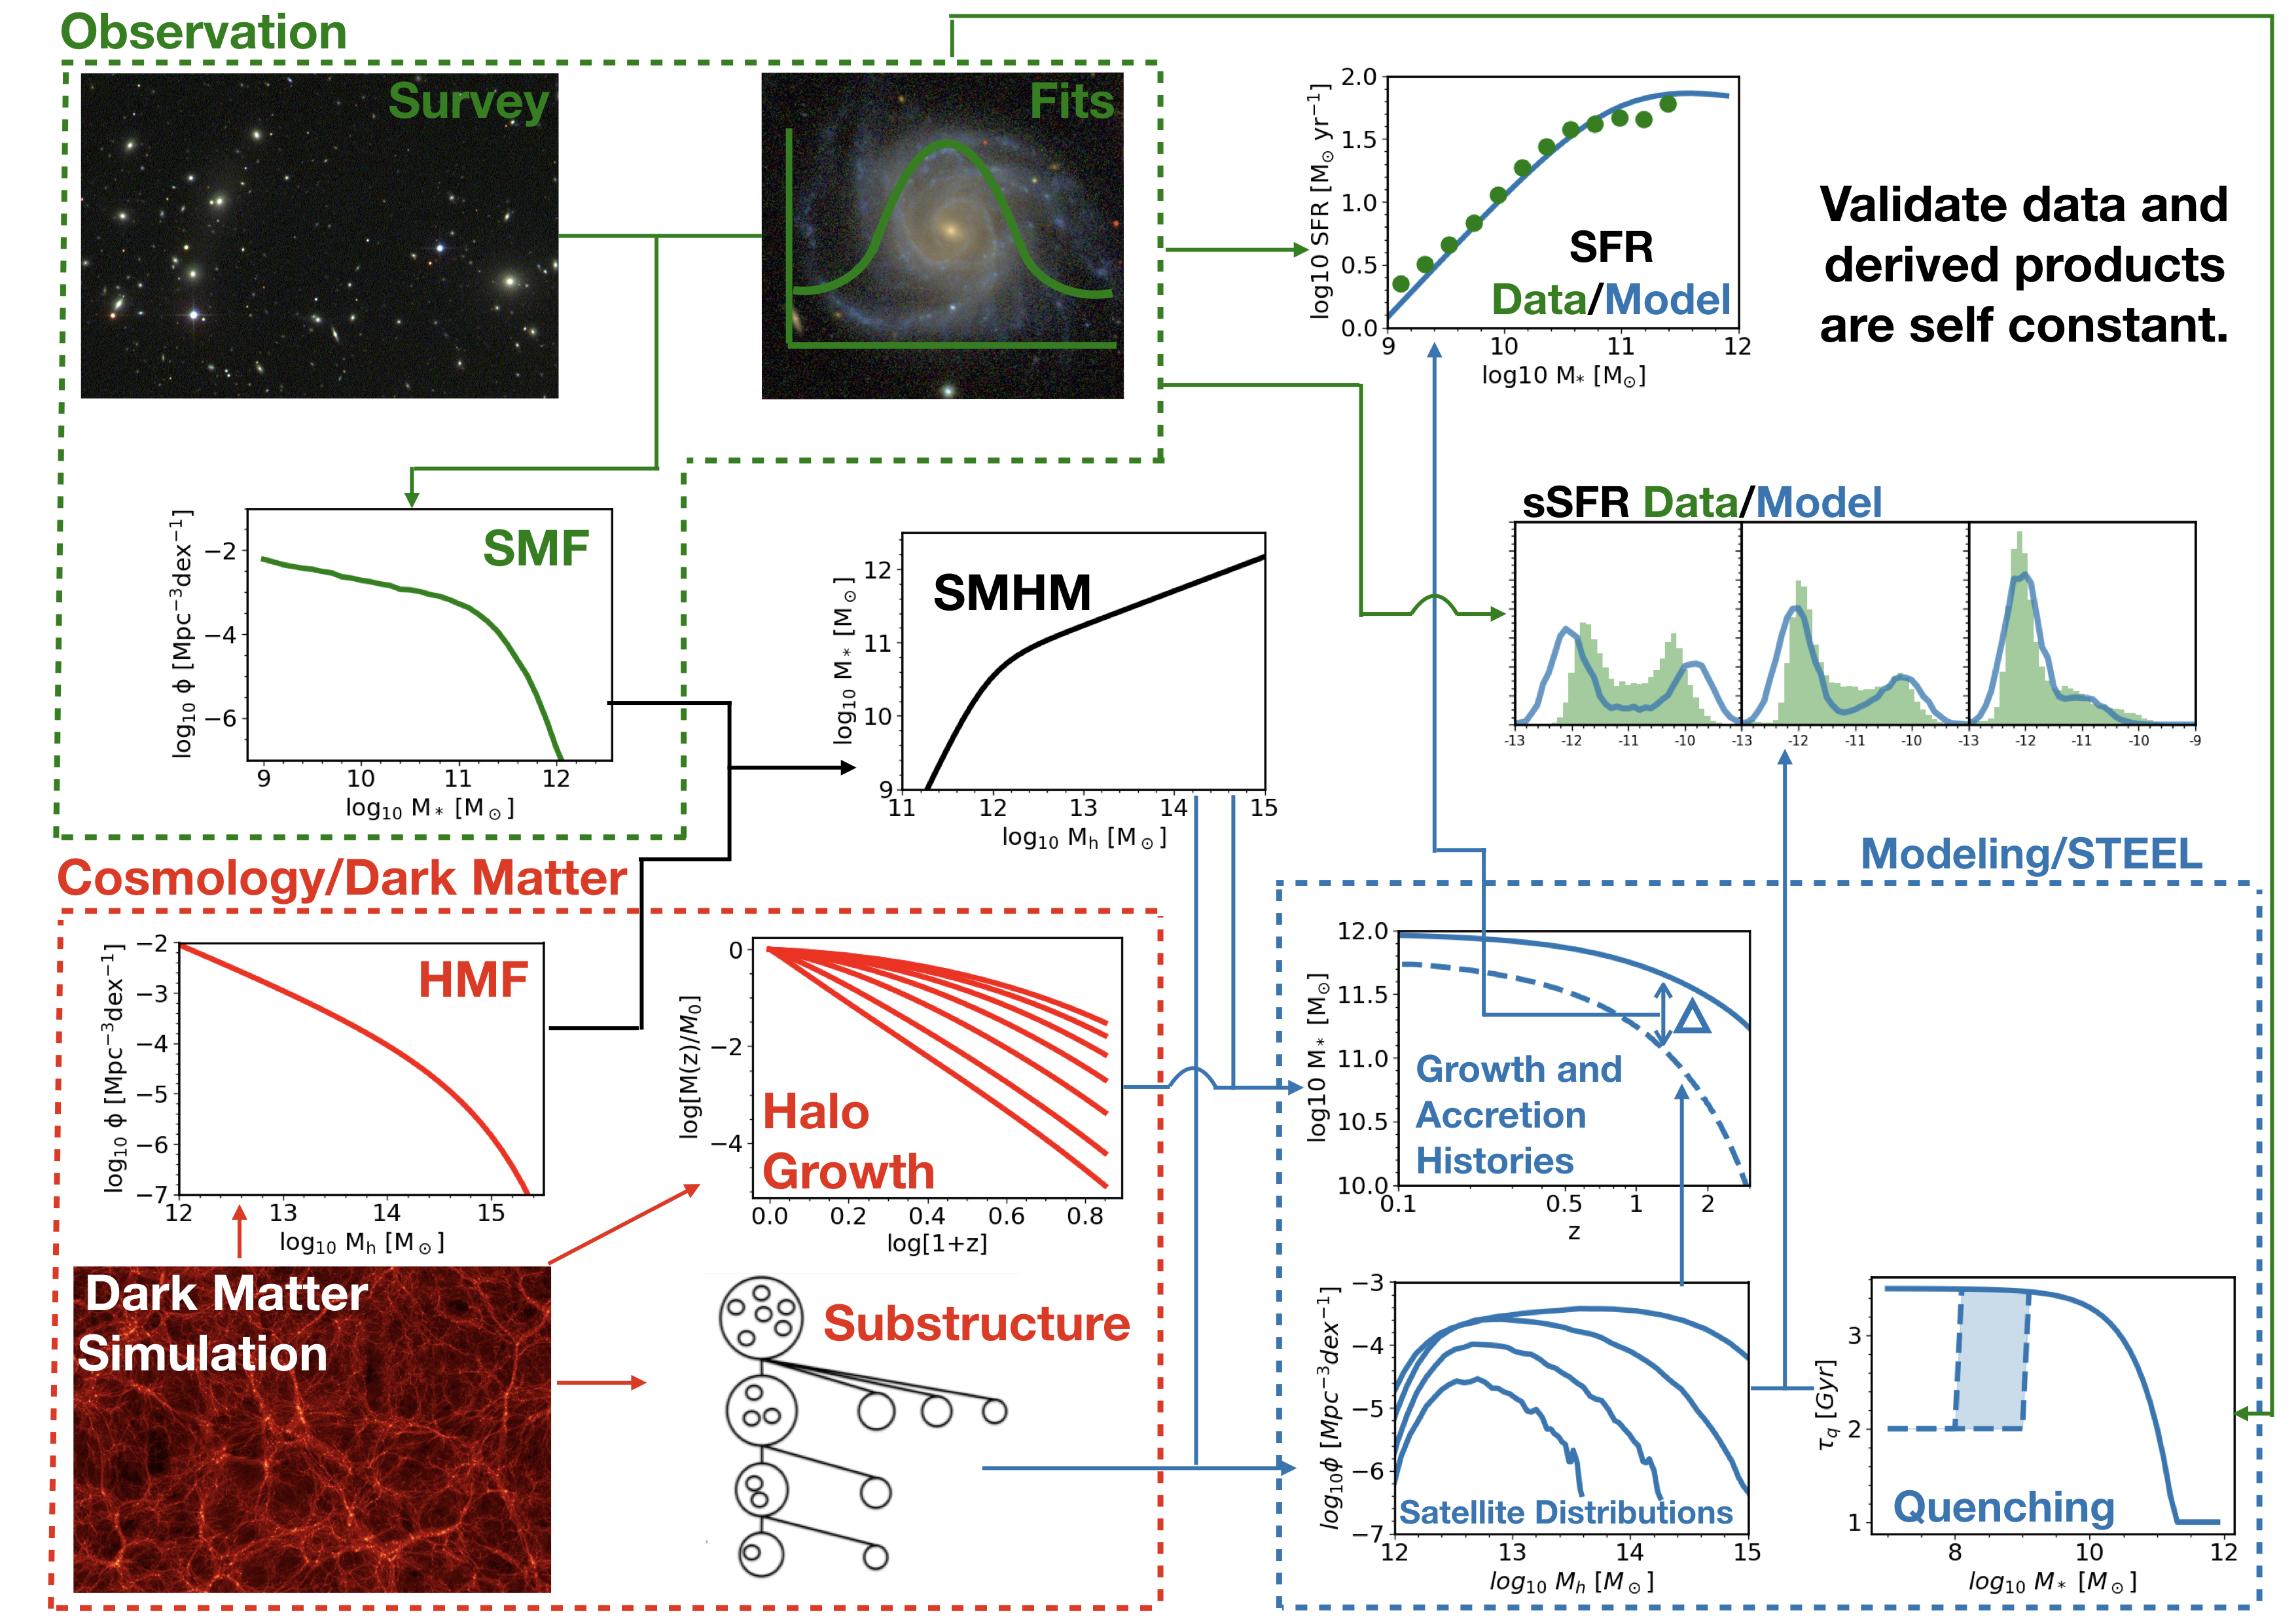
\includegraphics[width = \linewidth]{Figures/Chapter6/FullModelCartoon.png}
    \caption{Schematic cartoon related to Figure \ref{fig:SFRDerevation_Cartoon} of how \steel can be used to check self-consistency between fitting models used on observed data and the theoretical assumptions that underpin the fitting models.}
    \label{fig:Full_Mod_Toon}
\end{figure}
Items closer to the top of the list are less effected by the modelling and therefore likely to be more robust within this method. Often the empirical technique draws on observation to inform modelling, for example the quenching model from \citet{Wetzel2013GalaxyUniverse}, therefore this approach may well present an iterative loop. Using this approach any mismatch between the observational fit and the modelled property can be addressed from three angles appreciating the uncertainties inherent in fitting, modelling, and cosmology together.

\subsection{Galaxy modelling tool}

The proposition for \steel, or another statistical semi empirical model, to become a staple amoungst other competitive galactic modelling tools is based exclusively on the concept of a statistical dark matter accretion history. This is due to two factors; firstly the ability to simulate without volume or resolution, until computational power is so cheap that volume and resolution become non-issues a statistical model will have a place to match the rarest features in observation; secondly, the removal of discrete objects allows for a new type of continuity check where the consistency of a population is modelled as a priority over the consistency of an individual halo/galaxy. 

\steel is an excellent start to statistical semi-empirical modelling, however, it contains remnants of its proof of concept, the development of the proficiency of PJG in research, and code implementation and architecture. \steel was fully rewritten once during this Ph.D. and stands to be fully revised again. With any revision the model should be updated in the following ways,

\begin{itemize}
    \item The statistical dark matter accretion history should be a separate library, containing flexible cosmology, halo definitions (e.g. virial, splash-back, m200c, e.t.c...), and should be built in an object oriented fashion such that it is easily extendable.
    \item The galaxy modelling should be redesigned such that each dark matter accretion history is built upon using explicit probability distribution convolutions.
    \item The outputs should be shaped by the statistical dark matter accretion history and contain structured probability distributions to be able to post-process a hierarchical complexity of result.
    \item The post-processing suit should contain any and all integrators required to process the outputs into galaxy populations for cosmological volumes, single mass tracks, or given mass ranges.
    \item The post-processing suit should offer `views' on the data structure using flexible plotting routines for ease of query and graph creation by a non expert user simmilar to the API provided to IllustrisTNG \cite[][https://www.tng-project.org/data/vis/]{Nelson2019TheRelease} as well as a more complex return structure to extract the full data products.
\end{itemize}

As detailed in the PERT chart in Appendix \ref{Appx:HF}, this would take six months to one year of full time development depending on the programming and empirical modelling skills of the developer. Once developed, documented, and deployed such a tool would be of enormous value to the galactic astrophysics community. 

\section{In closing}

The applications of \steel detailed in Section \ref{sec:Future} each independently represent a tool that if correctly developed and made publicly available would be at the cutting edge of galactic astrophysics. The work done in this thesis represents the foundations upon which these tools can be built. 

In brief the findings from this thesis are: 
\begin{itemize}
    \item The dark matter structure and dynamics is the first order driver for prediction of galaxy properties including, satellite distributions, star formation rate, galaxy morphologies. 
    \item Assumptions made during stellar mass estimation produce significant non-trivial systematics in the pair fraction of galaxies and likely further properties, and without proper appreciation of such systematics we are likely to fundamentally misinterpret the nature of galaxy assembly. 
    \item Stellar mass functions with an enhanced number densities of high mass galaxies are in much better agreement with \LCDM cosmology than those with lower number densities of high mass galaxies. Furthermore, some traditional stellar mass functions are fundamentally incompatible with \LCDM hierarchical cosmology.
\end{itemize}

Dark matter dominating the evolution of galaxies is understood and the contributions made are novel but not unexpected. The source and complexities of the systematics in the pair fraction represent something that once known seems trivial but to the knowledge of PJG and coauthors FS and CC (an expert in galactic pair fractions) has not been addressed before from a quantitative theoretical standpoint. Finally, the lack of self-consistency between hierarchical \LCDM assembly and some stellar mass functions is a result of fundamental importance to galactic astrophysics. This result can only be reproduced from an approach that looks at the statistics of galactic populations and not discrete objects. It hints at a potentially devastating departure between observation and theory that if left unaddressed will hinder our understanding of the evolution of galaxies for the foreseeable future.
